
\chapter{Fundamentação Teórica}
\label{chap:fundamentacao}

Neste capítulo, são apresentados os conceitos que servem de insumo para a elaboração das etapas seguintes desse trabalho. Na seção \ref{sec:complexidade} são demostrados alguns conceitos necessários para identificar e classificar a complexidade de um algoritmo. A seção \ref{sec:pd} explica o básico sobre programação dinâmica, seus principais termos e o conceito de otimização, que servirá de base para a elaboração dos capítulos seguintes. Por fim, no capítulo \ref{sec:ensino} é feita uma análise de alguns trabalhos relacionados com o ensino de programação.



\section{Complexidade de Algoritmos}
\label{sec:complexidade}
Na ciência da computação, analisar um algoritmo está relacionado com a identificação da quantidade de recursos necessários para sua execução, podendo ser a quantidade de memória utilizada, largura de banda de comunicação, hardware do computador. Porém mais frequentemente a preocupação maior é em se medir o tempo computacional gasto para realizar determinado código \cite{Cormen09a}.

Quando é feita a análise de complexidade, é possível identificar qual classe um determinado algoritmo pertence. A tabela \ref{tab:classes} lista algumas classes de forma ordenada, sendo a primeira função a melhor possível e a última a pior. Após classificar um algoritmo, é possível escolher entre diversas soluções para um mesmo problema, qual é a mais adequada no momento e poder saber antes de executar quanto tempo e memória o algoritmo irá gastar quando o tamanho da entrada for $n$, onde $n$ corresponde, geralmente a quantidade de elementos que devem processados. Na figura \ref{fig:complexity} é possível observar o comportamento de algumas funções na medida que a quantidade de elementos aumenta.


\begin{table}[H]
	\centering
	\caption[Principais classes de funções para analisar algoritmos]{Principais classes de funções para analisar algoritmos}
	\label{tab:classes}
	\begin{tabular}{c|c}
		\hline \SPACE
		\textbf{Notação} & \textbf{Exemplo de algoritmos} \\ \hline \SPACE
		$O(1)$ & Determinar se um número é par ou ímpar \\ \hline \SPACE
		$O(log n)$ & Busca binária \\ \hline \SPACE
		$O(\sqrt{n})$ & Determinar se um número é primo \\ \hline \SPACE
		$O(n)$ & Procurar um elemento em um \textit{array} não ordenado \\ \hline \SPACE
		$O(n * log n)$ & \textit{Merge sort}\protect\footnotemark \\ \hline \SPACE
		$O(n^2)$ & \textit{Bubble sort}\protect\footnotemark \\ \hline \SPACE
		$O(n^3)$ & \textit{Floyd-Warshall}\protect\footnotemark \\ \hline \SPACE
		$O(n^c)$ & Encontrar o maior emparelhamento em um grafo \\ \hline \SPACE
		$O(c^n)_{c > 1}$ & Resolver o problema do caixeiro viajante\protect\footnotemark com programação dinâmica \\ \hline \SPACE
		$O(n!)$ & Resolver o problema do caixeiro viajante com força bruta \\ \hline
	\end{tabular}

	\fonte{Pr\'oprio Autor.}
\end{table}
\addtocounter{footnote}{-3}
\footnotetext{Ver mais em: http://quiz.geeksforgeeks.org/merge-sort/}
\addtocounter{footnote}{1}
\footnotetext{Ver mais em: http://quiz.geeksforgeeks.org/bubble-sort/}
\addtocounter{footnote}{1}
\footnotetext{Ver mais em: http://www.geeksforgeeks.org/dynamic-programming-set-16-floyd-warshall-algorithm/}
\addtocounter{footnote}{1}
\footnotetext{Ver mais em: http://www.geeksforgeeks.org/travelling-salesman-problem-set-1/}

\begin{figure}[H]
	\centering
	\caption[Gráfico das principais classes de complexidade]{Gráfico das principais classes de complexidade}
	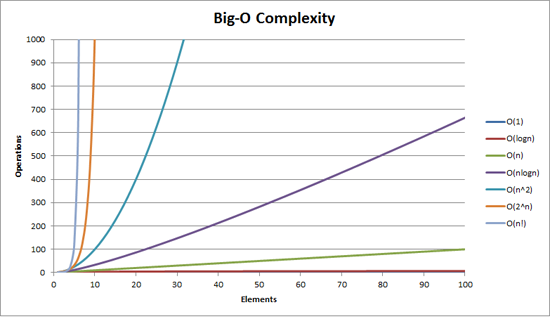
\includegraphics[width=0.7\textwidth]{complexity.png} % <- formatos PNG, JPG e PDF
	\fonte{PERRETT, 2010\nocite{Perrett2010}}
	\label{fig:complexity}
\end{figure}

\section{Programação dinâmica}
\label{sec:pd}

Programação dinâmica é uma técnica que combina soluções de subproblemas, da mesma maneira que a divisão e conquista, que divide o problema em subproblemas, resolve cada um recursivamente e depois é feita a junção das soluções para resolver o problema original. Porém este método é normalmente utilizado quando os subproblemas se sobrepõem, ou seja, um mesmo estado é encontrado diversas vezes na etapa de divisão. Portanto, se fosse aplicado um algoritmo ingênuo de divisão e conquista, um mesmo estado seria resolvido várias vezes, aumentando o custo computacional do algoritmo \cite{Cormen09a}. 

Para resolver o problema de sobreposição, a técnica de programação dinâmica salva a resposta de todos os estados que vão sendo encontrados. Assim, no momento que se deparar com algo que já foi resolvido ela simplesmente retorna o valor que já estava armazenado. 

A sequência de Fibonacci é um exemplo de fácil entendimento de quando é necessário a utilização de programação dinâmica. Esta é uma sequência de números inteiros que tem seu início com 0 e 1, os termos subsequentes são uma soma dos dois últimos números. A sequência recebeu o nome do matemático Leonardo de Pisa, mais conhecido como Fibonacci, que no ano de 1202 descreveu o crescimento da população de coelhos utilizando esta sequência \cite{LiveScience2013}. Os primeiros termos são:
\begin{equation}
0, 1, 1, 2, 3, 5, 8, 13, 21, 34, 55, 89, 144, 233, 377, 610, ...
\label{eq:fib}
\end{equation}
podendo ser representada através da seguinte recorrência, onde $fib(i)$ representa $i$-ésimo termo da sequência:
\begin{equation}
fib(i)=
\begin{cases}
i &\text{se } i \leq{1},\\
fib(i - 1) + fib(i - 2) &\text{se } i > {1}.
\end{cases}
\label{eq:fibrecorrence}
\end{equation}

\begin{figure}[H]
	\centering
	\caption[Árvore de recursão do Fibonacci de 5]{Árvore de recursão do Fibonacci de 5}
	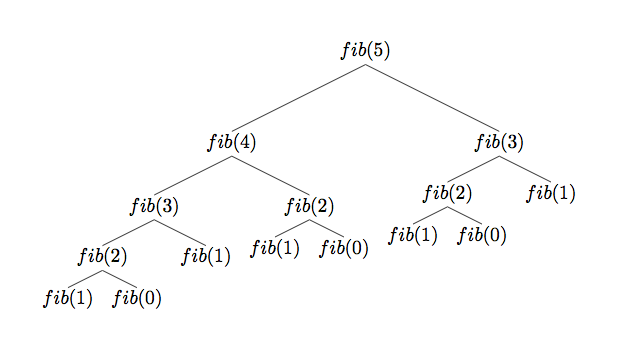
\includegraphics[width=0.7\textwidth]{fib5.png} % <- formatos PNG, JPG e PDF
	\fonte{SCHWARTZ, 2011\nocite{Schwartz2011}}
	\label{fig:fib5}
\end{figure}


Na figura \ref{fig:fib5} é apresentada a árvore de recursão gerada ao utilizar a equação \ref{eq:fibrecorrence} para o cálculo do $fib(5)$. Através dela, é fácil ver que diversos estados estão se repetindo, por exemplo: $fib(2)$ aparece três vezes e sempre que é encontrado ele é divido no $fib(1)$ e $fib(0)$, assim deixando a  complexidade deste algoritmo em $O(2^{N})$. Ao aplicar programação dinâmica neste algoritmo é possível reduzir a complexidade para $O(N)$, pois cada estado será expandido uma única vez.

O código a seguir mostra como seria a implementação da função sem a utilização de programação dinâmica.
\begin{lstlisting}[caption={Implementação Fibonacci sem programação dinâmica},label={lst:fibsimples}]
int fib(int i){
	if(i <= 1)
		return i;
	return fib(i - 1) + fib(i - 2);
}

\end{lstlisting}

Para otimizar o código e utilizar programação dinâmica basta incluir uma tabela que salva todos os estados. Sua inclusão faz uma alteração mínima no código, como é mostrado no algoritmo \ref{lst:fibpd}.

\textcolor{red}{Encontrar uma melhor forma de apresentar o novo código, mostrando as principais mudanças feitas para transformar o Algoritmo 1 no Algoritmo 2}

\begin{lstlisting}[caption={Implementação Fibonacci com programação dinâmica},label={lst:fibpd}]
#define MAX 20 // Valor maximo que sera consultado na funcao fib(i)
int tabela[MAX + 1]; // Tabela que guarda a resposta dos estados
					 // Inicialmente todos elementos recebem um valor nulo
					 // Para o problema do Fibonacci o valor nulo pode ser -1
					 
int fib(int i){
	if(tabela[i] != -1) // Verifica se ja foi calculado esse estado
		return tabela[i];
	if(i <= 1)
		return tabela[i] = i;
	// Resolve o estado, salva na tabela e o retorna
	return tabela[i] = fib(i - 1) + fib(i - 2);
}
\end{lstlisting}

Para mais informações sobre programação dinâmica e suas técnicas, o site \textit{TopCoder}\footnote{https://www.topcoder.com/community/data-science/data-science-tutorials/} possui um artigo amplo com vários problemas e dicas para soluções. Ele divide sua explicação em teoria e prática, começando nos tópicos mais simples e indo até alguns mais avançados.

\subsection{Otimizações}

Ao utilizar programação dinâmica para otimizar um problema, normalmente ocorre uma queda drástica na classe de complexidade associada a solução, como é o caso da sequência de Fibonacci, discutida na seção \ref{sec:pd}, onde foi possível sair de uma complexidade exponencial para uma linear. Apesar de parecer uma ótima forma de solucionar um problema, às vezes apenas aplicar programação dinâmica não é suficiente, e existem casos onde é possível e necessário otimizar ainda mais.

Para utilizar uma técnica de otimização de programação dinâmica, alguns critérios em relação a função de recorrência devem ser correspondidos. Cada técnica tem uma abordagem que possibilita a resolução de um conjunto de problemas que compartilham certas propriedades.

\textcolor{red}{Gostei do exemplo! Só adaptaria um pouco o texto, para deixar claro que você só está dando UM exemplo, para ilustrar o que seriam otimizações. Como está, parece que você já vai começar a explicar todas as otimizações.}

Dentre as otimizações disponíveis, as que envolvem redução de memória são as mais simples de serem aplicadas, seu uso pode ser facilmente entendido no problema da mochila \footnote{http://www.geeksforgeeks.org/dynamic-programming-set-10-0-1-knapsack-problem/}. Esse problema deseja maximar o valor dos itens colocados em uma mochila, onde estes possuem um valor e um peso associado, enquanto a mochila possui uma capacidade máxima de peso. Além disso, nenhum item pode ser dividido.  

\begin{equation}
dp[i][j] = 
\begin{cases}
0 &\text{se } i = 0 \text{ ou } j = 0,\\
max(valor[i-1] + dp[i-1][j-peso[i-1]], dp[i-1][j]) &\text{se } peso[i-1] \leq{j},\\
dp[i-1][j] &\text{se } peso[i-1] > j
\end{cases}
\label{eq:knapsack}
\end{equation}

O problema da mochila pode ser resolvido através da relação de recorrência apresentada acima, onde $dp[i][j]$ representa o valor máximo que pode se conseguir ao colocar os $i$-ésimos primeiros itens em uma mochila de capacidade $j$. Os vetores $valor$ e $peso$, representam o valor e peso associado a cada um dos $n$ itens, respectivamente. A resposta para o problema estará em $dp[n][capacidade]$.
 
Analisando a complexidade da equação \ref{eq:knapsack} é fácil ver que será necessário $O(n*capacidade)$, tanto de memória, quanto de tempo. Porém, é notório que para solucionar a linha $i$ da matriz de programação dinâmica, só são necessárias as respostas que já foram calculadas na linha $i - 1$, portanto podemos trabalhar apenas com duas linhas consecutivas da matriz, sempre alternando entre linha par e ímpar. 

\begin{equation}
dp[i\&1][j] = 
\begin{cases}
0 &\text{se } i = 0 \text{ ou } j = 0,\\

max(valor[i-1] + dp[\text{\textasciitilde}i\&1][j-peso[i-1]], dp[\text{\textasciitilde}i\&1][j]) &\text{se } peso[i-1] \leq{j},\\
dp[\text{\textasciitilde}i\&1][j] &\text{se } peso[i-1] > j
\end{cases}
\label{eq:knapsackmemorialinear}
\end{equation}

A equação \ref{eq:knapsackmemorialinear} demostra como reduzir a memória. Os valores que serão utilizados nas linhas da DP serão sempre 0 ou 1, assim o total de memória necessária é de $2*capacidade$, deixando com uma complexidade de $O(capacidade)$. A resposta para o problema da mochila utilizando esta relação estará em $dp[n\&1][capacidade]$.

No capítulo \ref{chap:desenvolvimento} serão apresentadas diversas técnicas, que poderão ser utilizadas tanto para redução de memória, quanto na redução de tempo de execução.

\section{Ensino de algoritmos}
\label{sec:ensino}

Nesta seção, são apresentados trabalhos que demostram alguns estudos de como construir um material didático, ou realizar o ensino de programação, que têm relação com o que neste está sendo desenvolvido. Dentre eles, é dada uma maior atenção aos que são apresentados nas subseções \ref{subsec:vihavainen} e \ref{subsec:methods}, pois estes apresentam metodologias que mais se adequam na proposta deste trabalho. 


\subsection{New Approaches and Tools in Teaching Programming} \nocite{newapproach}

Se propõe em criar uma ferramenta que facilite o aprendizado de linguagens de programação básicas, como C++, ao invés da utilização de\sigla{IDE}{Integrated Development Environment}(do inglês, \textit{Integrated Development Environment}). A finalidade desta ferramenta é ajudar os estudantes em não cometer erros que são comuns a quem está iniciando. Além disso, oferecer uma forma mais simples do professor auxiliar seus alunos.

\subsection{ICT Teaching Methods – Applications} \nocite{teachingapplications}

Realiza uma análise nos principais métodos e aplicações que auxiliam no aprendizado e no ensino dos tópicos de\sigla{ICT}{Information and Communication Technology}(do inglês, \textit{Information and Communication Technology}). Para cada método é exemplificado o seu funcionamento, como realizar a sua aplicação e para qual nível de estudante ele é mais apropriado. 


\subsection{ICT Teaching Methods – Programming Languages} \nocite{teachingapplicationslanguages}

Neste trabalho é feita uma análise semelhante a que foi realizada no trabalho apresentado na subseção anterior. Porém, o foco deste é o ensino de uma linguagem de programação, portanto os métodos apresentados demostram os passos ideais para transmitir os conceitos da linguagem proposta.

\subsection{A Survey of Literature on the Teaching of Introductory Programming} \nocite{Pears:2007:SLT:1345443.1345441}
 Foi desenvolvido um \textit{survey} que reúne algumas formas da literatura de ensinar a introdução de programação. Além disso, os trabalhos reunidos, foram classificados e agrupados pela forma de ensino e pelos métodos aplicados.

\subsection{Learning and Teaching Programming: A Review	and Discussion} \nocite{doi:10.1076/csed.13.2.137.14200} 
Uma ampla pesquisa na literatura com o foco na parte educacional do estudo de programação foi feita. Diversos métodos e tópicos foram identificados e analisados para poder ser realizado uma classificação, e assim, auxiliar os professores a identificar em seus alunos características comuns e padrões, que poderão ser contornados com base no que já foi realizado e está documentado na literatura.

\subsection{Extreme Apprenticeship Method in Teaching Programming for Beginners} \nocite{Vihavainen:2011:EAM:1953163.1953196}
\label{subsec:vihavainen}
Fala sobre como ensinar o básico de programação para quem está começando, ele propõe um modelo de ensino e mostra como esse método foi aplicado ao curso de ciência da computação.

\subsection{Methods of teaching programming} 
\nocite{methods}
\label{subsec:methods}
 Apresenta algumas metodologias de ensino de programação, mostrando quando e para qual nível de aluno cada metodologia pode ser aplicada. Estes métodos determinam a forma de estruturar o curso que deseja ser ensinado. 

	\textbf{Specification oriented:} Segundo o autor esse é um método adequado para quem tem uma base matemática e que está no 4º ou 5º ano de graduação. Este utiliza bastante a matemática, teoremas e algoritmos rígidos que são derivados diretamente da definição. 


 



